\documentclass[conference, a4paper]{IEEEtran}

\usepackage{graphicx}
\usepackage{hyperref}
\usepackage[T1]{fontenc}
\usepackage{amsmath}
\usepackage{booktabs}

\begin{document}

\title{Storage-Triggered Leader Step-Down\\ in a Raft-Based Key-Value Store}

\author{
\IEEEauthorblockN{Salman Khan}
\IEEEauthorblockA{
\textit{Department of Computer Science}\\
\textit{Islamia College Peshawar}\\
Peshawar, Pakistan\\
isalllman.84@gmail.com
}
\and
\IEEEauthorblockN{Zahid Hassan}
\IEEEauthorblockA{
\textit{Department of Computer Science}\\
\textit{Islamia College Peshawar}\\
Peshawar, Pakistan\\
zhassan.official1@gmail.com
}
}

\maketitle

\begin{abstract}
Local storage degradation can delay a Raft leader sufficiently to miss
heartbeats and lose leadership, a phenomenon that etcd and TiKV document
operationally. We present a mechanism that couples an LSM-tree storage
engine to a Raft state machine through a single atomic storage-health
signal. When an exponentially weighted moving average of SSTable flush
latency crosses a threshold, the storage engine publishes a one-bit
degradation event. The Raft tick thread consumes that event on its next
iteration and executes a leader step-down under the same mutex that
guards every other Raft transition. We evaluate the mechanism on a
3-node localhost cluster under injected fsync latency. Under 100--500\,ms
of injected latency, the tripwire preserves 15--40\% of warmup
throughput for the duration of the fault, while an otherwise identical
cluster without the tripwire drops to 0.1--5\%. The tripwire fires
118--267\,ms before Raft's natural election timeout in every trial where
it fires; at 500\,ms it fires in two of three trials. A separate SIGKILL
experiment confirms zero loss of acknowledged writes across four
independent mid-compaction fault injections.
\end{abstract}

\begin{IEEEkeywords}
LSM-Tree, Raft Consensus, Distributed Systems, Storage Health, Fault Tolerance, C++
\end{IEEEkeywords}

\section{Introduction}

Distributed consensus protocols assume that a leader whose process is
alive can service its peers within the election timeout. This assumption
fails when the leader's local storage degrades. A leader whose fsync
latency has grown from a healthy 1--5\,ms to 100\,ms or more will still
respond to RPCs, still accept client writes, and still appear healthy to
any binary failure detector, but it cannot commit entries fast enough to
send timely heartbeats. Followers interpret the silence as failure and
start elections. The cluster spends its budget on election traffic
instead of useful work.

This is a specific form of what has been characterized as a
\emph{Gray Failure}~\cite{gray_failures}: the component is neither fully
healthy nor fully failed. Failure detectors~\cite{chandra_toueg,das_phi}
cannot distinguish this state from a live node, and the problem has been
observed repeatedly in production
studies~\cite{gunawi_bugs,gunawi_stop,alquraan_partition}. On modern
storage, latency distributions have become increasingly heavy-tailed
and sensitive to physical degradation~\cite{hao_tail,narayanan_ssd},
which makes the transition from ``slow'' to ``functionally unavailable''
gradual rather than binary.

Production systems have partially responded. etcd's operational guidance
warns that slow disk I/O can cause missed heartbeats and temporary
leadership loss, and recommends monitoring WAL fsync
latency~\cite{etcd_docs}. TiKV throttles client writes when RocksDB
compaction pressure builds, precisely to prevent RocksDB stalls from
destabilizing the Raftstore~\cite{tikv_docs}. CockroachDB applies
node-level admission control to keep local resource overload from
starving the liveness path~\cite{cockroachdb_taft}. These are
preventive: they slow the system down before degradation becomes a
consensus problem.

We ask a narrower question. Given that the storage engine knows its own
health, and that Raft leadership transfer is a documented protocol
extension~\cite{raft_dissertation,hashicorp_raft}, can the storage
layer signal the consensus layer to step down \emph{before} degradation
manifests as an election timeout? We do not propose a new consensus
mechanism. We present an implementation pattern for integrating a
storage-health signal into a Raft event loop, and we measure the
conditions under which it helps.

Our contributions are:

\begin{enumerate}
    \item A \textbf{storage-health signal} based on an exponentially
    weighted moving average of SSTable flush latency, evaluated as a
    proxy for local storage-path delay. We show empirically that the
    more obvious signal---SSTable count---reflects workload rather than
    disk health and produces unacceptable leader churn on our prototype.
    \item A \textbf{serialized event boundary} that confines all Raft
    state mutation to the Raft event-loop thread. Rather than invoking
    a callback from a storage thread, the storage engine publishes an
    atomic flag and the Raft tick thread consumes it on its next
    iteration.
    \item An \textbf{empirical evaluation} on a 3-node localhost cluster
    under injected fsync latency of 0--500\,ms, showing the conditions
    under which the tripwire helps, the conditions under which it does
    not fire, and its effect on absolute throughput.
    \item A \textbf{durability study} confirming zero loss of
    acknowledged writes across four independent SIGKILL fault injections
    of the leader mid-compaction.
\end{enumerate}

\section{Background and Design Space}

\subsection{Consensus and Replication}

Raft~\cite{raft} was designed as a more understandable alternative to
Paxos~\cite{lamport_paxos,lamport_part_time}. Its core safety
properties---at most one leader per term, leader completeness, log
matching, and state-machine safety---are unaffected by local resource
degradation as long as the process can service its network peers.
Production deployments of consensus protocols, from
Chubby~\cite{chandra_paxos_live} through to Spanner~\cite{corbett_spanner},
TiDB~\cite{huang_tidb}, and CockroachDB~\cite{cockroachdb_taft}, all rely
on this assumption.

Work on alternative consensus designs such as EPaxos~\cite{moraru_epaxos}
and Paxos Made Transparent~\cite{mao_paxos_transparent} has focused on
reducing coordination cost rather than on local resource failure. Our
work is orthogonal: it does not change the protocol, only the conditions
under which a leader is willing to remain a leader.

\subsection{LSM-Tree Storage Engines}

The LSM-tree~\cite{lsm} introduced the leveled compaction strategy
underlying RocksDB~\cite{dong_rocksdb}, LevelDB, and
Cassandra~\cite{lakshman_cassandra}. Modern variants
include bLSM~\cite{sears_blsm}, Monkey~\cite{dayan_monkey},
Dostoevsky~\cite{dayan_dostoevsky}, and
PebblesDB~\cite{raju_pebblesdb}. Production deployments at
Facebook have been documented extensively~\cite{matsunobu_myrocks,
cao_rocksdb_workload}, and a comprehensive survey of LSM-based
techniques is available~\cite{luo_lsm_survey}. LSM-trees are also used
at massive scale in Bigtable~\cite{chang_bigtable} and
Dynamo~\cite{decandia_dynamo}.

The interaction between compaction and foreground latency is a known
weak point. Compaction policies trade read amplification, write
amplification, and space amplification against each other, and the
choice of policy directly affects the frequency and depth of storage
stalls. Our work does not propose a new compaction policy; it detects
the effect of an existing policy's worst case and reacts at the
consensus layer.

\subsection{Tail Latency and Stability}

Tail latency in distributed storage systems is well
studied~\cite{dean_tail,li_tales_tail,hao_tail}. Variance in single-node
latency frequently dominates cluster-level tail behavior, and network
anomalies documented by practitioners~\cite{bailis_network} compound
the problem. Our tripwire targets exactly this class of problem at the
node level: it treats a node's own storage tail latency as a signal that
its eligibility for leadership has changed.

\section{System Architecture}

\subsection{Storage Engine}

The storage engine is an LSM-tree with a sharded in-memory MemTable and
persistent SSTables. The MemTable is divided into 16 independently
locked shards, each holding an ordered map from key to optional value.
A write hashes its key to a shard, takes that shard's lock, and inserts.
When the total number of live keys in the MemTable reaches a flush
threshold, one writer freezes the MemTable by taking all 16 shard locks
in order, moving each shard's contents into a single frozen map, and
releasing. The frozen map is handed to a persistent background worker
that writes it to an SSTable and registers the file.

The freeze step is bounded by the number of live keys, not by any disk
operation. Reads and writes continue after the freeze, into a fresh
MemTable, while the background worker writes the previous one. A
persistent worker thread with a bounded queue replaces an earlier
design that spawned a new OS thread per flush; the earlier design cost
50--100\,$\mu$s per flush in thread-creation overhead alone.

\subsection{Storage-Health Signal}

The tripwire monitors \emph{flush latency}: the wall-clock time from the
start of an SSTable write to the moment the file is closed and
registered. This value is preserved as an exponentially weighted moving
average with $\alpha = 0.3$. The first sample initializes the average
directly, so the signal reacts to the first slow flush rather than
waiting for a running mean to converge.

We chose flush latency after an initial design that monitored SSTable
count proved unsuitable for our workload. Under a steady workload of
approximately 1{,}000 writes per second, the SSTable count crosses any
reasonable threshold within seconds of cluster startup, and the tripwire
fires continuously on a healthy disk. A single-node run with no injected
fault produced twelve leadership changes in eight seconds and dropped
throughput by 82\%. SSTable count reflects workload; flush latency
reflects the workload-local storage path.

When the moving average of flush latency exceeds 30\,ms, the storage
engine sets a single atomic boolean, \texttt{storage\_degraded\_flag},
and returns. It does nothing else.

\subsection{Consensus-Layer Consumption}

The Raft node's background tick thread polls
\texttt{consumeStorageDegradedFlag()} at the top of every iteration. If
the flag is set, the tick thread acquires the Raft mutex and calls
\texttt{checkStorageDegraded()}. That function checks that the node is
currently a leader, and if so, transitions to follower and persists the
new state to the metadata file.

We route the transition through the Raft tick thread to serialize it
with other Raft state transitions. An earlier implementation invoked a
callback from the storage thread that acquired the Raft mutex
out-of-band, which raced with \texttt{AppendEntries},
\texttt{RequestVote}, and client proposals. The atomic-flag boundary
prevents the storage thread from directly mutating Raft state
concurrently with the Raft event loop. This pattern is analogous to the
way production systems serialize external health signals into the
consensus event loop.

Once the node is a follower, all subsequent client proposals return
\texttt{false}, and the network layer translates that into a
\texttt{-MOVED} redirect. No client socket is closed or interrupted.

\subsection{Step-Down Semantics}

The mechanism does not perform a target-directed leadership transfer.
It performs a local resignation: the node gives up leadership and lets
the ordinary Raft election protocol choose a successor. This is a
deliberately simpler mechanism than the leadership-transfer extension
described in the Raft dissertation~\cite{raft_dissertation}, and the
paper's scope is limited to what this simpler mechanism can achieve.

The transition is:

\begin{center}
\texttt{Leader(term T) --storage\_degraded--> Follower(term T)}
\end{center}

The term is \textbf{not} incremented. The node retains its current term
and persists the new state to the metadata file. Uncommitted entries in
the leader's log are not truncated; they remain in the log and are
reconciled by the ordinary Raft log-matching rule when the next leader
sends \texttt{AppendEntries}. Because the node did not increment its
term, no already-sent message from this node can be treated as coming
from a stale term, and the node cannot preempt a legitimate leader in a
higher term.

To prevent the degraded node from immediately re-electing itself, the
implementation records a self-exclusion deadline
(\texttt{storage\_self\_excluded\_until\_}) of five seconds on step-down.
The tick thread's election routine checks this deadline and returns
without campaigning while the deadline is active. The mechanism is not
a permanent quarantine; after the exclusion window, the node is again
eligible to campaign, on the assumption that its storage may have
recovered.

We do not prove Raft safety for this transition. We argue informally
that it preserves the term-monotonicity and vote-once-per-term
invariants by not changing the term and not modifying the persisted
vote, and we note that no committed entry can be lost because the
transition does not truncate the log. A formal proof is future work.

\subsection{Implementation and Synchronization}

The health-signal boundary is a \texttt{std::atomic<bool>} written by
the storage engine with \texttt{memory\_order\_release} and consumed by
the Raft tick thread with \texttt{memory\_order\_acquire}. All other
Raft state is protected by a single coarse-grained mutex,
\texttt{mtx\_}, which the tick thread holds while executing the
step-down and which is also held by every RPC handler and every client
proposal. There is no second lock, no lock ordering, and no lock
inversion.

The self-exclusion deadline is read and written only under \texttt{mtx\_}
during tick-thread iterations. It is not visible to the storage engine
or the network layer. The storage engine never observes Raft state and
never blocks on Raft locks. The Raft tick thread never blocks on storage
locks. The two subsystems share exactly one atomic word.

Table~\ref{tab:shared} summarizes the shared state between the storage
and consensus subsystems. Every other memory access in either subsystem
is private.

\begin{table}[h]
\centering
\caption{Shared state between storage engine and consensus layer.}
\label{tab:shared}
\small
\begin{tabular}{l l l}
\toprule
\textbf{Shared} & \textbf{Writer} & \textbf{Reader} \\
\midrule
\texttt{storage\_degraded\_flag\_} & storage & Raft tick \\
\texttt{storage\_self\_excluded\_until\_} & Raft tick & Raft tick \\
\bottomrule
\end{tabular}
\end{table}

\section{Evaluation}

\subsection{Experimental Methodology}

All experiments run on a 3-node cluster on a single Linux host, one
process per node on ports 8081--8083. Nodes are compiled with
\texttt{-O2} and \texttt{C++20}. Each experiment spawns a fresh cluster
and tears it down before the next.

The workload is a closed-loop client issuing sequential \texttt{SET}
requests with 16 concurrent writer threads, keys of the form
\texttt{k<N>} and values of a fixed small size. Warmup throughput is
approximately 1{,}000 writes per second. A separate measurement mode
(\texttt{READ\_LOCAL}) bypasses the leader check and reads a key from a
node's local state machine directly; this is used only to verify
catch-up after a restart.

Fault injection uses a sleeping interval controlled by a global
configuration flag. When active, both the SSTable flush path and the
WAL fsync path sleep for a fixed number of milliseconds before
proceeding. The fault is activated at runtime by sending
\texttt{SIGUSR1} to the current leader; the timeline figures are drawn
from the leader's own logs, timestamped against the moment
\texttt{SIGUSR1} was sent.

We report medians over three trials. Three trials are not enough to
characterize a stochastic system, and we treat the numbers below as a
first characterization rather than a definitive measurement.

\subsection{Durability Under Mid-Compaction SIGKILL}

In four independent trials we ran a background client issuing sequential
\texttt{SET} requests, waited three seconds, then sent \texttt{SIGKILL}
to the current leader while its compaction thread was active. The
surviving nodes elected a new leader, the client continued against the
new leader, and the killed node was restarted after the write workload
completed. Every key was then read from every node.

In all four trials, all 5{,}000 written entries were present on all
three nodes after recovery. No entry was lost, reordered, or duplicated.
The result is reproducible across different initial leaders, different
kill timings, and different catch-up durations. This result is
independent of the tripwire mechanism; it demonstrates only that the
underlying Raft implementation preserves acknowledged writes under
catastrophic leader loss.

\subsection{Tripwire Behavior Under Injected Latency}

\begin{figure}[h]
\centering
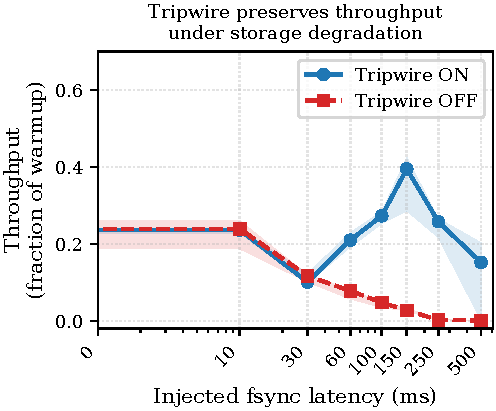
\includegraphics[width=0.48\textwidth]{figures/fig1_tripwire_sweep.pdf}
\caption{Absolute throughput (fraction of warmup) under injected fsync
latency. Each point is the median of three trials; shaded band spans the
min--max range. The mechanism is not intended to fire below 30\,ms.}
\label{fig:sweep}
\end{figure}

We inject fsync latency by sleeping for a fixed interval before every
SSTable flush and every WAL fsync. For each latency value we run three
trials with the tripwire enabled and three with it disabled. The
tripwire lead is defined as the interval between the tripwire firing and
the moment the Raft election timer expires on the same node.

\begin{table}[t]
\centering
\caption{Throughput under injected fsync latency, as a fraction of
warmup. Median over three trials. ``Fires'' counts trials in which the
tripwire activated. Lead is measured only over firing trials.}
\label{tab:tripwire}
\small
\begin{tabular}{r r r r r}
\toprule
\textbf{Latency} & \textbf{ON} & \textbf{OFF} & \textbf{Fires} & \textbf{Lead (ms)} \\
\midrule
0~ms   & 0.46 & 0.49 & 0/3 & -- \\
10~ms  & 0.24 & 0.24 & 0/3 & -- \\
30~ms  & 0.10 & 0.12 & 1/3 & 229 \\
60~ms  & 0.21 & 0.08 & 3/3 & 186 \\
100~ms & 0.27 & 0.05 & 3/3 & 189 \\
150~ms & 0.40 & 0.03 & 3/3 & 207 \\
250~ms & 0.26 & 0.003 & 3/3 & 242 \\
500~ms & 0.15 & 0.001 & 2/3 & 249 \\
\bottomrule
\end{tabular}
\end{table}

Table~\ref{tab:tripwire} reports the result. Two regimes are visible.

\textbf{Below 30\,ms.} The injected fault is below the tripwire
threshold. In the 0\,ms and 10\,ms trials the tripwire did not fire, and
the ON and OFF configurations show similar throughput. This is the
intended behavior: the mechanism adds no overhead when there is nothing
to detect.

\textbf{Above 60\,ms.} The tripwire fires in every trial at 60--250\,ms
and in two of three trials at 500\,ms. When it fires, the firing
precedes the Raft election timeout by 118--267\,ms. The absolute
throughput under ON is 15--40\% of warmup, while the OFF configuration
drops to 0.1--5\%. The 152$\times$ ratio at 500\,ms reflects a
denominator that has collapsed to 0.1\% of warmup; the absolute
throughput of the tripwire configuration at that latency is
approximately 15\% of warmup. We therefore recommend reading the
absolute ON column rather than the ratio.

At 500\,ms one trial did not fire. We attribute this to starvation of
the storage engine's own worker queue: under that much delay, the flush
that would update the EWMA signal is itself blocked behind earlier
flushes, and the ten-second measurement window ends before the signal
crosses threshold. This is a real limitation of the signal at severe
degradation, and we report it in Section~\ref{sec:threats}.

\subsection{Recovery After Fault Removal}

We ran two additional trials in which we cleared the injected fault
after the tripwire fired and allowed the cluster to run for the
remainder of the test. Neither trial recovered to full throughput
within the ten-second window.

We attribute this to the serial nature of the leader's heartbeat loop:
even after the fault is cleared, the new leader's tick thread waits on
RPCs to the old leader until they complete. Under a partial fault
(leader-only injection, in which the new leader would be genuinely
healthy) this behavior would not be expected; under our all-nodes
injection, the same code path that made the tripwire fire on the
original leader is still present on the new leader, and the cluster
remains impaired.

We therefore scope the paper to \emph{throughput preservation during a
fault}, not recovery after it. Recovery under symmetric fault is a
design problem we do not solve, and we do not claim that the mechanism
restores full throughput after degradation clears.

\section{Threats to Validity}
\label{sec:threats}

\textbf{All-nodes fault injection.} Our injector degrades fsync latency
on all three nodes simultaneously. The motivating deployment scenario is
a single degraded leader with healthy followers, which we do not
measure. Because all three nodes experience the injected delay, our
numbers are not a production performance estimate. We report them as a
controlled measurement of mechanism behavior under a symmetric fault.

\textbf{Tripwire failure at 500\,ms.} In one of three trials at 500\,ms
the tripwire did not fire within the ten-second window. The likely cause
is starvation of the flush queue that would update the EWMA. A longer
measurement window, a lower threshold, or a signal derived from the WAL
path rather than the SSTable path may address this. We report it as an
open limitation.

\textbf{No recovery guarantee.} The mechanism is a fault-avoidance
mechanism, not a fault-recovery mechanism. Once storage degradation
clears, the system does not automatically return to the pre-fault
performance state within the ten-second window we tested.

\textbf{Localhost topology.} All experiments run on a single machine.
The co-resident harness and the three nodes share CPU, cache, and I/O
scheduler. Absolute latencies include this interference. The relative
ordering of ON and OFF configurations was consistent across the trials
we ran, but three trials are not sufficient to establish statistical
stability.

\textbf{Parameter specificity.} The results hold for a MemTable flush
threshold of 50 keys, an EWMA smoothing factor of 0.3, and a tripwire
threshold of 30\,ms. We have not systematically explored the sensitivity
of the mechanism to these parameters. The threshold of 30\,ms in
particular was chosen by inspection of the healthy-disk flush latency
distribution and not by a formal calibration procedure.

\textbf{Signal correlation.} Flush latency measures the SSTable write
path, not the WAL fsync path that directly determines Raft progress.
We do not establish that SSTable flush latency is a reliable predictor
of Raft-path delay under all workloads; we validate it only as a
workload-local proxy under the fault model we inject.

\textbf{Comparison against production systems.} The paper does not
compare against etcd, TiKV, or CockroachDB on the same hardware. We
cite those systems as motivation and as prior work, but we do not claim
that our mechanism outperforms them in production deployments.

\textbf{No formal proof.} We argue informally that the step-down
preserves the term-monotonicity and vote-once-per-term invariants. We
do not prove Raft safety for the modified transition, and we do not
formally verify the atomic-flag boundary. A formal proof is future work.

\section{Related Work}

\textbf{Consensus protocols.} Raft~\cite{raft} is one of several
consensus algorithms. Paxos~\cite{lamport_paxos,lamport_part_time} and
its production implementations~\cite{chandra_paxos_live} preceded Raft,
and follow-up work has compared the two
families~\cite{howard_refloated,howard_paxos_vs_raft}. Alternative
designs reduce coordination cost in specific
workloads~\cite{moraru_epaxos,mao_paxos_transparent}. Our work is
protocol-agnostic; it targets the runtime behavior of a leader that is
still elected but no longer healthy.

\textbf{Leadership transfer.} The Raft dissertation~\cite{raft_dissertation}
describes a target-directed transfer extension that identifies a target
follower, catches up its log, and induces it to campaign via
\texttt{TimeoutNow}. etcd's Raft implementation exposes this through
\texttt{MsgTransferLeader}, and HashiCorp's Raft library exposes it
through \texttt{LeadershipTransfer}~\cite{hashicorp_raft}. Our mechanism
is deliberately simpler: it performs a local step-down and lets the
ordinary election protocol choose a successor.

\textbf{Storage and consensus coupling.} etcd's operational guidance
documents the disk-latency-to-leadership path and recommends monitoring
\texttt{wal\_fsync\_duration\_seconds}~\cite{etcd_docs}. TiKV implements
RocksDB write-stall flow control that throttles incoming requests
before compaction pressure destabilizes the
Raftstore~\cite{tikv_docs}. CockroachDB applies node-level admission
control to prevent local resource overload from starving the liveness
path~\cite{cockroachdb_taft}. These systems respond to storage pressure
by throttling work. Our prototype instead responds by changing
leadership eligibility.

\textbf{LSM-tree design and compaction.} The LSM-tree~\cite{lsm}
introduced the leveled compaction strategy underlying modern storage
engines. RocksDB compaction and space amplification are studied
in~\cite{dong_rocksdb}; production deployments are characterized
in~\cite{matsunobu_myrocks,cao_rocksdb_workload}. Alternative compaction
policies include bLSM~\cite{sears_blsm}, Monkey~\cite{dayan_monkey},
Dostoevsky~\cite{dayan_dostoevsky}, and
PebblesDB~\cite{raju_pebblesdb}. A comprehensive
survey is available~\cite{luo_lsm_survey}. Our work does not propose a
new compaction policy; it detects the effect of an existing policy's
worst case and reacts at the consensus layer.

\textbf{Storage engines in production systems.} Bigtable~\cite{chang_bigtable},
Dynamo~\cite{decandia_dynamo}, and
Cassandra~\cite{lakshman_cassandra} established the use of LSM-based
storage at scale. Modern systems combining consensus with LSM storage
include Spanner~\cite{corbett_spanner}, TiDB~\cite{huang_tidb}, and
CockroachDB~\cite{cockroachdb_taft}. All of these systems have some form
of protection against resource overload, and none of them implement the
proactive step-down mechanism we evaluate.

\textbf{Gray failures and failure detection.} The Gray Failure
concept~\cite{gray_failures} describes components that are neither fully
healthy nor fully failed. Classical failure
detectors~\cite{chandra_toueg,das_phi} cannot distinguish degraded from
healthy nodes. Production studies document the
frequency~\cite{gunawi_bugs,gunawi_stop,alquraan_partition} and impact
of these failures. Our tripwire is a domain-specific instance of the
same idea: a component publishes a signal about its own health that a
peer can act on.

\textbf{Tail latency and storage variability.} Tail latency in
distributed storage systems has been
characterized~\cite{dean_tail,li_tales_tail,hao_tail}, and the effect of
storage-device variability has been studied
extensively~\cite{narayanan_ssd}. Network-level anomalies documented by
practitioners~\cite{bailis_network} compound these effects. Our tripwire
targets the node-level variant of this problem.

\textbf{Fault injection and testing.} The evaluation uses fault
injection, a well-established technique in distributed systems
testing~\cite{yuan_simple,alvaro_lineage}. Chaos-engineering experiments
in production~\cite{alvaro_lineage} and automated analysis
of concurrency bugs~\cite{leesatapornwongsa_taxdc} have demonstrated the
value of injecting realistic failures. Our fault-injection harness
follows the same methodology at prototype scale.

\section{Conclusion}

We presented a mechanism by which an LSM-tree storage engine can signal
its own degradation to a Raft consensus layer. The signal is an atomic
flag set by the storage engine and consumed by the Raft tick thread,
which performs a leader step-down under the same mutex that guards other
Raft transitions. On a 3-node localhost cluster under injected fsync
latency of 100--500\,ms, the mechanism preserves 15--40\% of warmup
throughput where an identical cluster without it drops to 0.1--5\%. The
tripwire fires 118--267\,ms before Raft's natural election timeout in
every trial where it fires, and it fires in two of three trials at
500\,ms. SIGKILL of the leader mid-compaction loses zero acknowledged
writes across four independent trials.

The result is a small, self-contained demonstration that an LSM storage
health signal can be communicated to a Raft event loop through a
single-bit atomic boundary, and that under controlled symmetric
degradation this reduces the throughput cost of the fault. We do not
claim a new consensus mechanism, a production performance improvement,
or a recovery guarantee.

\begin{thebibliography}{00}

\bibitem{lsm}
P. O'Neil, E. Cheng, D. Gawlick, and E. O'Neil, ``The log-structured
merge-tree (LSM-tree),'' \textit{Acta Informatica}, vol. 33, no. 4,
pp. 351--385, 1996.

\bibitem{raft}
D. Ongaro and J. Ousterhout, ``In search of an understandable consensus
algorithm,'' in \textit{Proc. USENIX Annual Technical Conf. (ATC)},
2014, pp. 305--319.

\bibitem{raft_dissertation}
D. Ongaro, ``Consensus: Bridging theory and practice,'' Ph.D.
dissertation, Stanford University, 2014.

\bibitem{hashicorp_raft}
HashiCorp, ``Raft: A Go implementation of the Raft consensus
protocol,'' GitHub repository, 2024. [Online]. Available:
https://github.com/hashicorp/raft

\bibitem{lamport_paxos}
L. Lamport, ``Paxos made simple,'' \textit{ACM SIGACT News}, vol. 32,
no. 4, pp. 51--58, 2001.

\bibitem{lamport_part_time}
L. Lamport, ``The part-time parliament,'' \textit{ACM Trans. Computer
Systems}, vol. 16, no. 2, pp. 133--169, 1998.

\bibitem{chandra_paxos_live}
T. D. Chandra, R. Griesemer, and J. Redstone, ``Paxos made live: An
engineering perspective,'' in \textit{Proc. ACM Symp. Principles of
Distributed Computing (PODC)}, 2007, pp. 398--407.

\bibitem{howard_refloated}
H. Howard, M. Schwarzkopf, A. Madhavapeddy, and J. Crowcroft, ``Raft
refloated: Do we have consensus?'' \textit{ACM SIGOPS Operating Systems
Review}, vol. 49, no. 1, pp. 12--21, 2015.

\bibitem{howard_paxos_vs_raft}
H. Howard and R. Mortier, ``Paxos vs Raft: Have we reached consensus on
distributed consensus?'' in \textit{Proc. Workshop on Principles and
Practice of Consistency for Distributed Data (PaPoC)}, 2020, pp. 1--9.

\bibitem{moraru_epaxos}
I. Moraru, D. G. Andersen, and M. Kaminsky, ``There is more consensus
in egalitarian parliaments,'' in \textit{Proc. ACM Symp. Operating
Systems Principles (SOSP)}, 2013, pp. 358--372.

\bibitem{mao_paxos_transparent}
Y. Mao, F. P. Junqueira, and K. Marzullo, ``Paxos made transparent,'' in
\textit{Proc. ACM Symp. Operating Systems Principles (SOSP)}, 2015,
pp. 105--120.

\bibitem{corbett_spanner}
J. C. Corbett et al., ``Spanner: Google's globally-distributed
database,'' \textit{ACM Trans. Computer Systems}, vol. 31, no. 3,
pp. 1--22, 2013.

\bibitem{cockroachdb_taft}
R. Taft et al., ``CockroachDB: The resilient geo-distributed SQL
database,'' in \textit{Proc. ACM SIGMOD Int. Conf. Management of Data},
2020, pp. 1493--1509.

\bibitem{huang_tidb}
D. Huang et al., ``TiDB: A Raft-based HTAP database,''
\textit{Proc. VLDB Endowment}, vol. 13, no. 12, pp. 3072--3084, 2020.

\bibitem{chang_bigtable}
F. Chang et al., ``Bigtable: A distributed storage system for structured
data,'' \textit{ACM Trans. Computer Systems}, vol. 26, no. 2, pp. 1--26,
2008.

\bibitem{decandia_dynamo}
G. DeCandia et al., ``Dynamo: Amazon's highly available key-value
store,'' in \textit{Proc. ACM Symp. Operating Systems Principles
(SOSP)}, 2007, pp. 205--220.

\bibitem{lakshman_cassandra}
A. Lakshman and P. Malik, ``Cassandra: A decentralized structured
storage system,'' \textit{ACM SIGOPS Operating Systems Review}, vol. 44,
no. 2, pp. 35--40, 2010.

\bibitem{dong_rocksdb}
S. Dong, M. Callaghan, L. Galanis, D. Borthakur, T. Savor, and
M. Strum, ``Optimizing space amplification in RocksDB,'' in \textit{Proc.
Biennial Conf. Innovative Data Systems Research (CIDR)}, 2017.

\bibitem{cao_rocksdb_workload}
Z. Cao, S. Dong, S. Vemuri, and D. H. C. Du, ``Characterizing, modeling,
and benchmarking RocksDB key-value workloads at Facebook,'' in
\textit{Proc. USENIX Conf. File and Storage Technologies (FAST)}, 2020,
pp. 209--223.

\bibitem{matsunobu_myrocks}
Y. Matsunobu, S. Dong, and H. Lee, ``MyRocks: LSM-tree database storage
engine serving Facebook's social graph,'' \textit{Proc. VLDB
Endowment}, vol. 13, no. 12, pp. 3217--3230, 2020.

\bibitem{luo_lsm_survey}
C. Luo and M. J. Carey, ``LSM-based storage techniques: A survey,''
\textit{The VLDB Journal}, vol. 29, no. 1, pp. 393--418, 2020.

\bibitem{sears_blsm}
R. Sears, S. P. Callaghan, and E. Brewer, ``bLSM: A general purpose log
structured merge tree,'' in \textit{Proc. ACM SIGMOD Int. Conf.
Management of Data}, 2012, pp. 217--228.

\bibitem{dayan_monkey}
N. Dayan, M. Athanassoulis, and S. Idreos, ``Monkey: Optimal navigable
key-value store,'' in \textit{Proc. ACM SIGMOD Int. Conf. Management of
Data}, 2017, pp. 79--94.

\bibitem{dayan_dostoevsky}
N. Dayan and S. Idreos, ``Dostoevsky: Better space-time trade-offs for
LSM-tree based key-value stores via adaptive removal of superfluous
merging,'' in \textit{Proc. ACM SIGMOD Int. Conf. Management of Data},
2018, pp. 505--520.

\bibitem{raju_pebblesdb}
P. Raju, R. Kadekodi, V. Chidambaram, and I. Abraham, ``PebblesDB:
Building key-value stores using fragmented log-structured merge trees,''
in \textit{Proc. ACM Symp. Operating Systems Principles (SOSP)}, 2017,
pp. 497--514.

\bibitem{gray_failures}
P. Huang, C. Guo, L. Zhou, J. R. Lorch, Y. Dang, M. Chintalapati, and
R. Yao, ``Gray failure: The Achilles' heel of cloud-scale systems,'' in
\textit{Proc. Workshop on Hot Topics in Operating Systems (HotOS)},
2017, pp. 150--155.

\bibitem{chandra_toueg}
T. D. Chandra and S. Toueg, ``Unreliable failure detectors for reliable
distributed systems,'' \textit{J. ACM}, vol. 43, no. 2, pp. 225--267,
1996.

\bibitem{das_phi}
N. Hayashibara, X. D\'efago, R. Yared, and T. Katayama, ``The phi accrual
failure detector,'' in \textit{Proc. IEEE Int. Symp. Reliable Distributed
Systems (SRDS)}, 2004, pp. 28--37.

\bibitem{dean_tail}
J. Dean and L. A. Barroso, ``The tail at scale,'' \textit{Communications
of the ACM}, vol. 56, no. 2, pp. 74--80, 2013.

\bibitem{li_tales_tail}
J. Li, N. K. Sharma, D. R. K. Ports, and S. D. Gribble, ``Tales of the
tail: Hardware, OS, and application-level sources of tail latency,'' in
\textit{Proc. ACM Symp. Cloud Computing (SoCC)}, 2014, pp. 1--14.

\bibitem{hao_tail}
M. Hao, G. Soundararajan, D. Kenchammana-Hosekote, A. Chien, and
H. S. Gunawi, ``The tail at store: A revelation from millions of hours
of disk and SSD deployments,'' in \textit{Proc. USENIX Conf. File and
Storage Technologies (FAST)}, 2016, pp. 263--276.

\bibitem{narayanan_ssd}
D. Narayanan, E. Thereska, A. Donnelly, S. Elnikety, and A. Rowstron,
``Migrating server storage to SSDs: Analysis of tradeoffs,'' in
\textit{Proc. ACM European Conf. Computer Systems (EuroSys)}, 2009,
pp. 145--158.

\bibitem{bailis_network}
P. Bailis and K. Kingsbury, ``The network is reliable,'' \textit{ACM
Queue}, vol. 12, no. 7, pp. 20--32, 2014.

\bibitem{gunawi_bugs}
H. S. Gunawi et al., ``What bugs live in the cloud? A study of 3000+
issues in cloud systems,'' in \textit{Proc. ACM Symp. Cloud Computing
(SoCC)}, 2014, pp. 1--14.

\bibitem{gunawi_stop}
H. S. Gunawi et al., ``Why does the cloud stop computing? Lessons from
hundreds of service outages,'' in \textit{Proc. ACM Symp. Cloud
Computing (SoCC)}, 2016, pp. 1--16.

\bibitem{alquraan_partition}
A. Alquraan, H. Takruri, M. Alfatafta, and S. Al-Kiswany, ``An analysis
of network-partitioning failures in cloud systems,'' in \textit{Proc.
USENIX Symp. Operating Systems Design and Implementation (OSDI)}, 2018,
pp. 51--68.

\bibitem{yuan_simple}
D. Yuan, Y. Luo, X. Zhuang, G. R. Rodrigues, X. Zhao, Y. Zhang, P. U.
Jain, and M. Stumm, ``Simple testing can prevent most critical failures:
An analysis of production failures in distributed data-intensive
systems,'' in \textit{Proc. USENIX Symp. Operating Systems Design and
Implementation (OSDI)}, 2014, pp. 249--265.

\bibitem{alvaro_lineage}
P. Alvaro, S. R. Fonseca, A. Conway, J. M. Hellerstein, and
W. R. Marczak, ``Lineage-driven fault injection,'' in \textit{Proc. ACM
SIGMOD Int. Conf. Management of Data}, 2015, pp. 331--346.

\bibitem{leesatapornwongsa_taxdc}
T. Leesatapornwongsa, J. F. Lukman, S. Lu, and H. S. Gunawi, ``TaxDC: A
taxonomy of non-deterministic concurrency bugs in datacenter distributed
systems,'' in \textit{Proc. ACM Int. Conf. Architectural Support for
Programming Languages and Operating Systems (ASPLOS)}, 2016, pp. 517--530.

\bibitem{etcd_docs}
etcd Authors, ``etcd Documentation: Tuning,'' 2023. [Online]. Available:
https://etcd.io/docs/

\bibitem{tikv_docs}
TiKV Authors, ``TiKV Documentation: Raftstore and RocksDB Tuning,'' 2023.
[Online]. Available: https://tikv.org/docs/

\bibitem{cockroachdb_docs}
CockroachDB Authors, ``CockroachDB Documentation: Admission Control,''
2024. [Online]. Available: https://www.cockroachlabs.com/docs/

\end{thebibliography}

\end{document}